\documentclass{article}
% generated by Madoko, version 1.1.6
%mdk-data-line={1}


\usepackage[heading-base={2},section-num={False},bib-label={hide},fontspec={True}]{madoko2}


\begin{document}



%mdk-data-line={6}
\mdxtitleblockstart{}
%mdk-data-line={6}
\mdxtitle{\mdline{6}The Second Day}%mdk
\mdxauthorstart{}
%mdk-data-line={11}
\mdxauthorname{\mdline{11}22 January 2019}%mdk
\mdxauthorend\mdtitleauthorrunning{}{}\mdxtitleblockend%mdk
\mdline{8}
\begin{mdtoc}%mdk

\section*{Contents}\label{sec-contents}%mdk%mdk

\begin{mdtocblock}%mdk

\mdtocitemx{sec-session-one}{\mdref{sec-session-one}{1.\hspace*{0.5em}Session One}}%mdk

\begin{mdtocblock}%mdk

\mdtocitemx{sec-can-maluss-law-be-verified-experimentally}{\mdref{sec-can-maluss-law-be-verified-experimentally}{1.1.\hspace*{0.5em}Can Malus’s law be verified experimentally?}}%mdk

\begin{mdtocblock}%mdk

\mdtocitemx{sec-procedure-practical-method}{\mdref{sec-procedure-practical-method}{1.1.1.\hspace*{0.5em}Procedure (Practical Method)}}%mdk

\mdtocitemx{sec-evaluation-of-procedure}{\mdref{sec-evaluation-of-procedure}{1.1.2.\hspace*{0.5em}Evaluation of Procedure}}%mdk

\mdtocitemx{sec-table-of-results}{\mdref{sec-table-of-results}{1.1.3.\hspace*{0.5em}Table of Results.}}%mdk

\mdtocitemx{sec-evaluation-of-readings}{\mdref{sec-evaluation-of-readings}{1.1.4.\hspace*{0.5em}Evaluation of Readings}}%mdk

\mdtocitemx{sec-analysis-of-readings}{\mdref{sec-analysis-of-readings}{1.1.5.\hspace*{0.5em}Analysis of Readings}}%mdk
%mdk
\end{mdtocblock}%mdk
%mdk
\end{mdtocblock}%mdk
%mdk
\end{mdtocblock}%mdk
%mdk
\end{mdtoc}%mdk

%mdk-data-line={10}
\section{\mdline{10}1.\hspace*{0.5em}\mdline{10}Session One}\label{sec-session-one}%mdk%mdk

%mdk-data-line={11}
\subsection{\mdline{11}1.1.\hspace*{0.5em}\mdline{11}Can Malus’s law be verified experimentally?}\label{sec-can-maluss-law-be-verified-experimentally}%mdk%mdk

%mdk-data-line={13}
\subsubsection{\mdline{13}1.1.1.\hspace*{0.5em}\mdline{13}Procedure (Practical Method)}\label{sec-procedure-practical-method}%mdk%mdk

%mdk-data-line={15}
\begin{enumerate}[noitemsep,topsep=\mdcompacttopsep]%mdk

%mdk-data-line={15}
\item\mdline{15}Set up the equipment with the white LED and two filters.%mdk

%mdk-data-line={16}
\item\mdline{16}Turn on the microcontroller, and set the filters to a 0 degrees offset.%mdk

%mdk-data-line={17}
\item\mdline{17}Record the initial intensity sensor value.%mdk

%mdk-data-line={18}
\item\mdline{18}Change the angle between the two filters in steps of 5 degrees, and record the intensity sensor value at each offset interval, being careful not to misalign the sensor or LED.%mdk

%mdk-data-line={19}
\item\mdline{19}Repeat steps 3 and 4 until a sufficient number of repeats has been obtained to reduce the impact of anomalous results.%mdk
%mdk
\end{enumerate}%mdk

%mdk-data-line={21}
\subsubsection{\mdline{21}1.1.2.\hspace*{0.5em}\mdline{21}Evaluation of Procedure}\label{sec-evaluation-of-procedure}%mdk%mdk

%mdk-data-line={23}
\noindent\mdline{23}This first method was easy to carry out once all the equiptment was aligned correctly, and the sensor placed over the center of the LED beam. Initially, two clamp stands were used for each of the polarising filters, and the primary filter was rotated in place. This, however, caused a cramped working space, causing the sensor to shift position.%mdk

%mdk-data-line={25}
\mdline{25}To combat this, I placed both the filters, sandwiched together, in the same clamp stand. For each offest interval, both filters were removed, rotated, and put back into place, carefully making sure that the filter covered all the beam.%mdk

%mdk-data-line={27}
\mdline{27}The LED beam also spread further than expected, reducing the intensity at the sensor. This was reduced by moving the components as close together as possible, but could have been entirely eliminated with the use of a laser.%mdk

%mdk-data-line={29}
\subsubsection{\mdline{29}1.1.3.\hspace*{0.5em}\mdline{29}Table of Results.}\label{sec-table-of-results}%mdk%mdk

%mdk-data-line={31}
\noindent\mdline{31}Table\mdline{31}~\mdref{results}{\mdcaptionlabel{1}}\mdline{31} shows the results of session one.%mdk

%mdk-data-line={33}
\begin{table}[tbp]%mdk
\begin{mdcenter}%mdk
\begin{mdtabular}{6}{\dimeval{(\linewidth)/6}}{1ex}%mdk
\begin{tabular}{lccccc}\cmidrule[\dimpx{2}]{2-2}\cmidrule[\dimpx{2}]{3-3}\cmidrule[\dimpx{2}]{4-4}\cmidrule[\dimpx{2}]{5-5}\cmidrule[\dimpx{2}]{6-6}
{\mdseries\mdline{35}Angle}&{\mdseries\mdline{35} Raw sensor output}&{\mdseries\mdline{35}}&{\mdseries\mdline{35}}&{\mdseries\mdline{35}}&{\mdseries\mdline{35}}\\
{\mdseries\mdline{36}}&{\mdseries\mdline{36} Repeat one}&{\mdseries\mdline{36} Repeat two}&{\mdseries\mdline{36} Repeat three}&{\mdseries\mdline{36} Average}&{\mdseries\mdline{36} Std Dev}\\

\midrule
\mdline{38} 0&\mdline{38} 1240&\mdline{38} 1121&\mdline{38} 1255&\mdline{38} 1205&\mdline{38} 73.4\\
\mdline{39} 5&\mdline{39} 1270&\mdline{39} 1105&\mdline{39} 1225&\mdline{39} 1200&\mdline{39} 85.3\\
\mdline{40} 10&\mdline{40} 1265&\mdline{40} 1077&\mdline{40} 1187&\mdline{40} 1176&\mdline{40} 94.4\\
\mdline{41} 15&\mdline{41} 1245&\mdline{41} 1022&\mdline{41} 1115&\mdline{41} 1127&\mdline{41} 112.0\\
\mdline{42} 20&\mdline{42} 1204&\mdline{42} 961&\mdline{42} 1036&\mdline{42} 1067&\mdline{42} 124.4\\
\mdline{43} 25&\mdline{43} 1151&\mdline{43} 887&\mdline{43} 949&\mdline{43} 996&\mdline{43} 138.0\\
\mdline{44} 30&\mdline{44} 1099&\mdline{44} 839&\mdline{44} 875&\mdline{44} 937&\mdline{44} 140.9\\
\mdline{45} 35&\mdline{45} 1030&\mdline{45} 751&\mdline{45} 773&\mdline{45} 851&\mdline{45} 155.1\\
\mdline{46} 40&\mdline{46} 971&\mdline{46} 636&\mdline{46} 655&\mdline{46} 754&\mdline{46} 188.1\\
\mdline{47} 45&\mdline{47} 841&\mdline{47} 561&\mdline{47} 514&\mdline{47} 639&\mdline{47} 176.8\\
\mdline{48} 50&\mdline{48} 697&\mdline{48} 448&\mdline{48} 465&\mdline{48} 539&\mdline{48} 139.1\\
\mdline{49} 55&\mdline{49} 571&\mdline{49} 398&\mdline{49} 366&\mdline{49} 445&\mdline{49} 110.3\\
\mdline{50} 60&\mdline{50} 451&\mdline{50} 278&\mdline{50} 303&\mdline{50} 344&\mdline{50} 93.5\\
\mdline{51} 65&\mdline{51} 321&\mdline{51} 203&\mdline{51} 195&\mdline{51} 240&\mdline{51} 70.6\\
\mdline{52} 70&\mdline{52} 222&\mdline{52} 141&\mdline{52} 120&\mdline{52} 161&\mdline{52} 53.9\\
\mdline{53} 75&\mdline{53} 130&\mdline{53} 83&\mdline{53} 62&\mdline{53} 92&\mdline{53} 34.8\\
\mdline{54} 80&\mdline{54} 64&\mdline{54} 38&\mdline{54} 34&\mdline{54} 45&\mdline{54} 16.3\\
\mdline{55} 85&\mdline{55} 17&\mdline{55} 16&\mdline{55} 9&\mdline{55} 14&\mdline{55} 4.4\\
\mdline{56} 90&\mdline{56} 1&\mdline{56} 1&\mdline{56} 1&\mdline{56} 1&\mdline{56} 0\\
\midrule[\dimpx{2}]
\end{tabular}\end{mdtabular}

%mdk-data-line={59}
\mdhr{}%mdk

%mdk-data-line={60}
\noindent\mdline{60}\mdcaption{\textbf{Table~\mdcaptionlabel{1}.}~\mdcaptiontext{Experiment 1 results}}%mdk
%mdk
\end{mdcenter}\label{results}%mdk
%mdk
\end{table}%mdk

%mdk-data-line={62}
\subsubsection{\mdline{62}1.1.4.\hspace*{0.5em}\mdline{62}Evaluation of Readings}\label{sec-evaluation-of-readings}%mdk%mdk

%mdk-data-line={64}
\noindent\mdline{64}These results follow exactly with the expected outcomes. The variation in initial values is due to changes in the distance between LED and sensor, and the different polarising filters used. The standard variation of the results is within acceptable ranges, but it is interesting to note that the standard deviation clearly increases towards the middle of the range of angles, and decreases again towards the end of the range. This is due to the change in starting intensity having little effect towards the extremes of intensity%mdk

%mdk-data-line={66}
\subsubsection{\mdline{66}1.1.5.\hspace*{0.5em}\mdline{66}Analysis of Readings}\label{sec-analysis-of-readings}%mdk%mdk

%mdk-data-line={68}
\noindent\mdline{68}To verify that these readings follow Malus\mdline{68}'\mdline{68}s law, we need to use the following substitutions:%mdk

%mdk-data-line={70}
\mdline{70}$I\propto\cos^2\theta$\mdline{70}%mdk

%mdk-data-line={72}
\mdline{72}$I=I_0\cos^2\theta$\mdline{72}%mdk

%mdk-data-line={74}
\mdline{74}$\Rightarrow y=mx+c$\mdline{74}%mdk

%mdk-data-line={76}
\mdline{76}$\therefore y=I, m=I_0, x=\cos^2\theta, c=0$\mdline{76}%mdk

%mdk-data-line={78}
\mdline{78}We can plot these values on a line graph:%mdk

%mdk-data-line={80}
\mdline{80}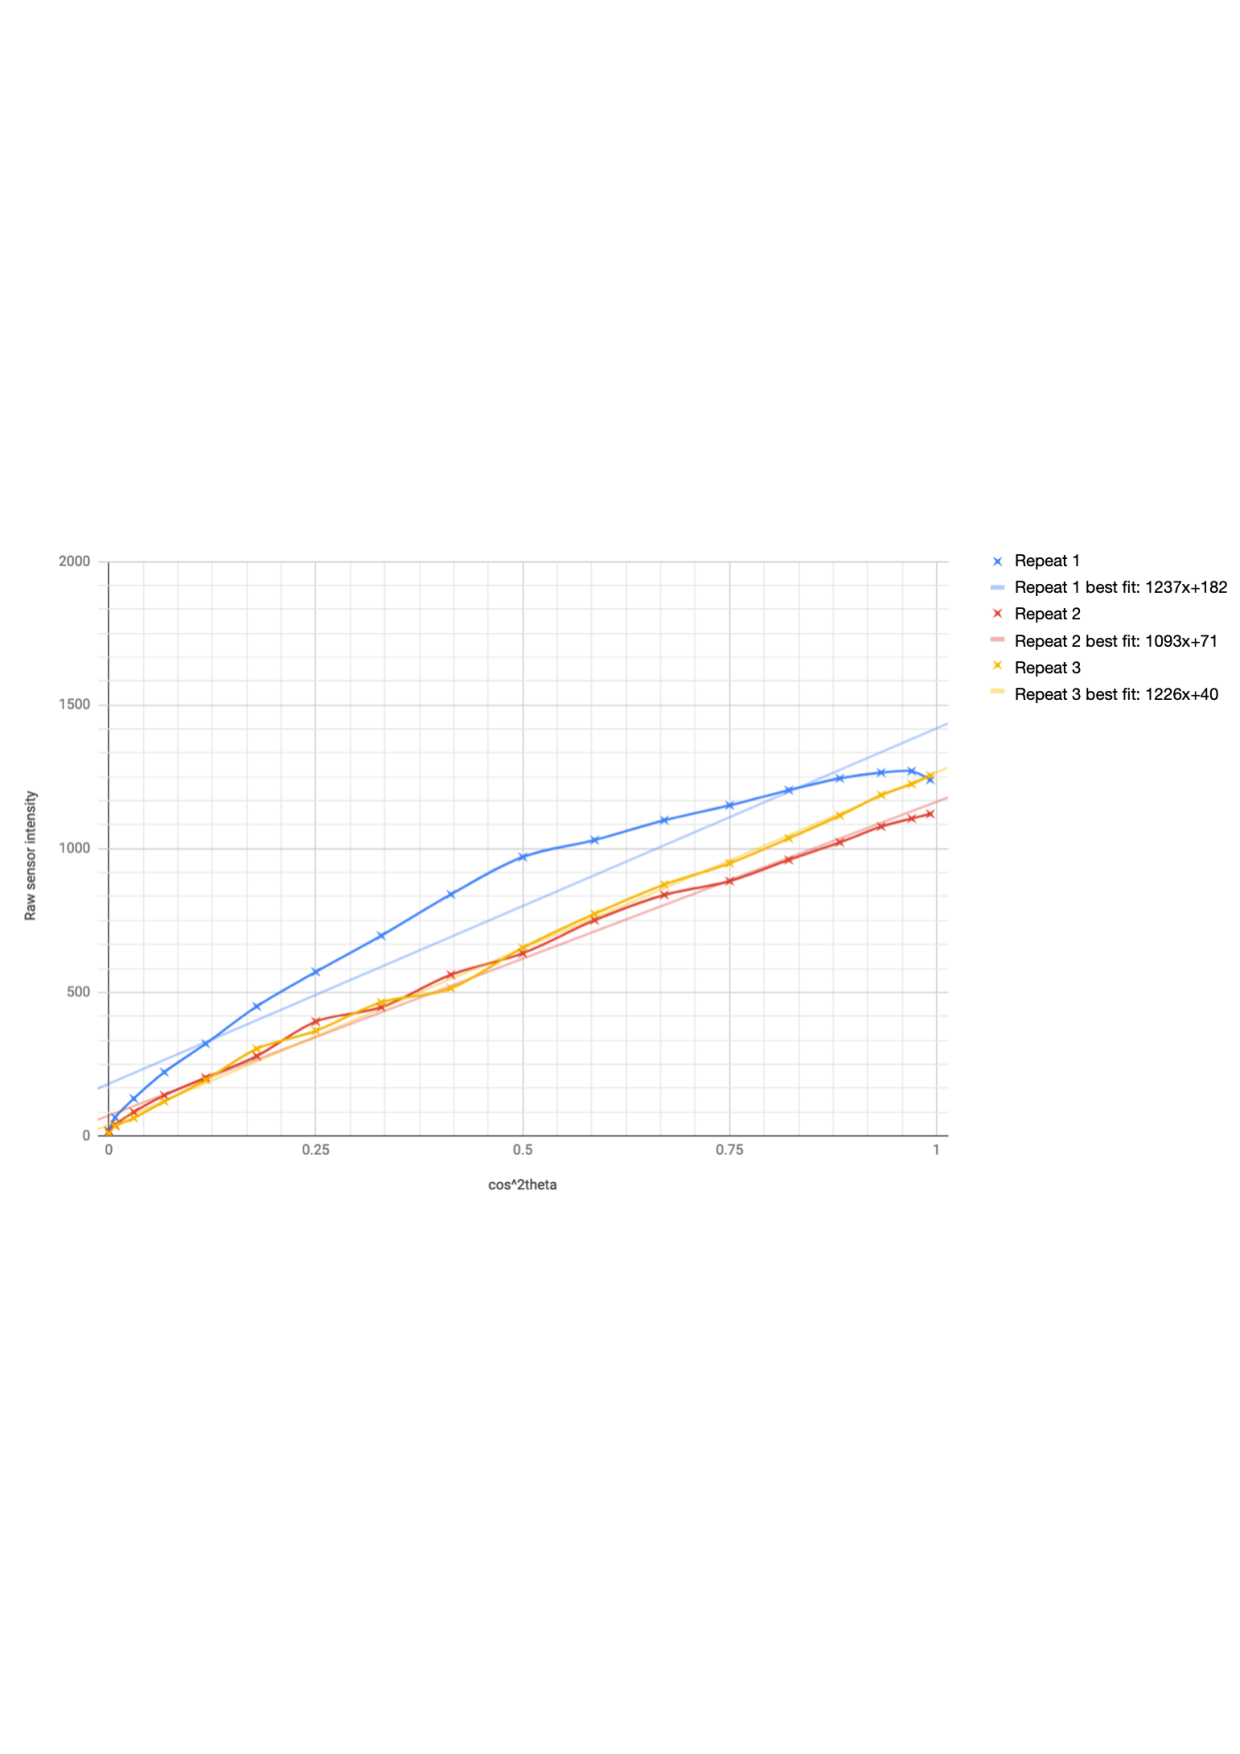
\includegraphics[keepaspectratio=true,width=\dimmin{}{\dimwidth{0.90}}]{images/Screenshot-2019-01-23-at-19.28.08}{}\mdline{80}%mdk%mdk


\end{document}
